\section{When Smoothness Is Rational: Descriptor-Driven Selective Prediction}
\label{sec:decision}

Where the oracle gap is non-positive, over-smoothing cannot be repaired, but the model can still report when its forecast is likely to degrade. We attach a shallow head (21K parameters, under 1\% of the backbone's) to the forecaster's last hidden state, trained jointly to predict structural descriptors of the future window: the probability and position of an imminent change point, ordinal bins of drift, volatility, and trend slope, and a five-dimensional spectral summary, all labeled for free from the future window at training time.

\paragraph{Descriptor supervision does not repair point accuracy at small scale.}
The head improves point MSE only marginally and only in specific cells---about one percent on PatchTST-ETTm1 at best, nothing reliable elsewhere, negative when fine-tuning a 48M foundation model (Appendix~\ref{app:negative}): most windows here sit in the rational-shrinkage regime, leaving representation shaping little bias to remove.

\paragraph{The descriptor output is a reliable forward-looking risk signal.}
The head's change-point output predicts the forecast's error: abstaining on the top quintile by predicted change-point probability reduces the remaining MSE by 2.7\% on ETTh1 and 5.3\% on ETTm1 (Figure~\ref{fig:riskcov}). The signal outperforms random ranking ($+0.2\%$), context-volatility ranking ($+0.4\%$/$+1.2\%$, actively harmful), and ranking by the true change-point label ($-1.6\%$/$-4.5\%$); against trained error-prediction baselines (ridge and MLP on context statistics, fit on validation) it wins on ETTh1 ($-0.3\%$ at best) and ties on ETTm1, requiring no validation data or extra training. The head's smoothed probabilities rank windows more reliably than the noisy realized labels, suggesting a generalizable structural signal rather than memorized targets (abstained windows fall back to a conservative forecaster or human review).

The signal transfers to a fine-tuned Chronos-Bolt at no extra cost: abstaining by predicted change-point probability reduces the remaining MSE by 3.6\% on ETTh1 and 9.6\% on ETTm1, the latter exceeding the oracle-volatility bound ($-7.5\%$), while context-volatility ranking is ineffective ($+1.3\%$): better backbones make the free signal more useful, not less.

\paragraph{Where the signal pays off.}
The head pays off exactly where risk is not visible from the context (Table~\ref{tab:decision}, Appendix~\ref{app:matrix}): its margin over the free context-volatility ranking is decisive where that baseline fails (Traffic: $+3.2\%$) and vanishes where the lookback already exposes the risk (Electricity; weather; Table~\ref{tab:decision}). The rule transfers across backbones: on a fine-tuned Chronos-Bolt, the volatility channel recovers $-3.2\%$ on Traffic where context volatility is harmful ($+2.9\%$), and on Electricity the free baseline again suffices ($-6.0\%$).

\begin{figure}[t]
  \centering
  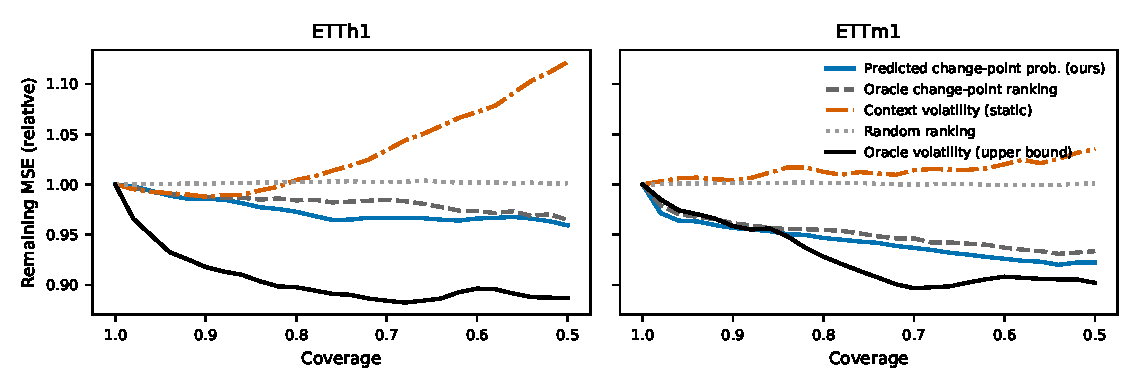
\includegraphics[width=0.55\linewidth]{figures/fig_riskcov.pdf}
  \caption{Risk--coverage curves on ETTh1, ETTm1, and fine-tuned Chronos-Bolt. Predicted change-point probability (blue) reduces remaining MSE monotonically, beating oracle change-point ranking (gray), context volatility (red), and random ranking (dashed); oracle volatility (black) marks the exploitable upper bound.}
  \label{fig:riskcov}
\end{figure}

